\chapter{\textbf{INTRODUCTION}}
Insérer ici un paragraphe intéressant global et accrocheur.

\begin{quote}
« All models are wrong, but some are useful.»\\
-- George Box
\end{quote}

\section{Mise en contexte}
Parler des modèles globaux d'écosystème (MGE).

\section{Le jeu de données}
\subsection{Nature des données}
Les données proviennent de l'étude de Jacquet.
\subsection{Distribution globale}
Voici la distribution globale des réseaux utilisés. 


\FloatBarrier
\begin{figure}[!htb]
\centering
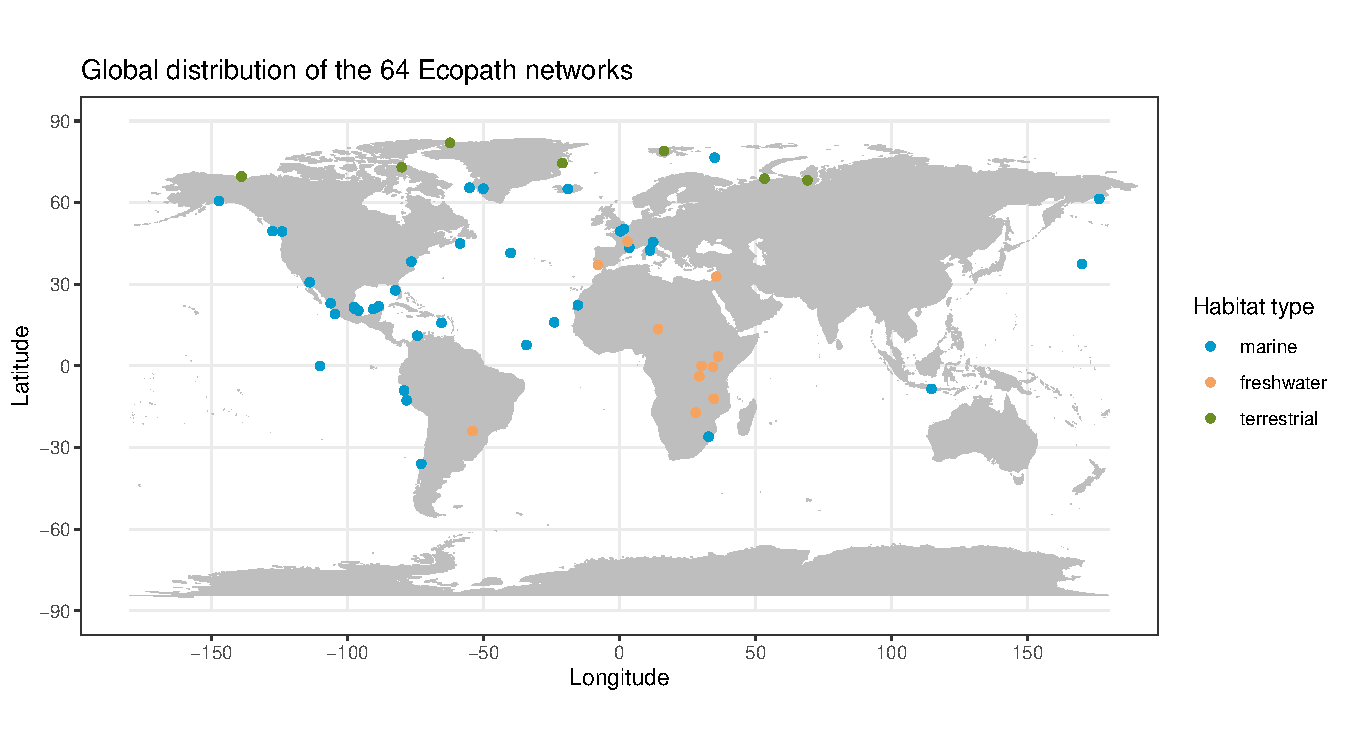
\includegraphics[width=\textwidth]{figs/chapitre1/network_map.pdf} % ici mettre le répertoire exact de la figure - Dossier Thèse, sous-dossier figs - chapitre 1
\caption[Titre de figure]{
Distribution des réseaux Ecopath \par{}
\smallskip		% saut de ligne entre titre et légende de figure
\normalfont{Légende de figure} 
}
\label{reaction_norms}
\end{figure}




% ajouté ceci pour faire un test 
% cite correctement dans le texte mais plus à la fin générale du document
%\singlespacing 
%{\renewcommand{\bibname}{References}
%\renewcommand{\bibsection}{\section{\bibname}}
%\bibliography{bib/library}}
%\bibliographystyle{styles/myBEAS} 
%
